% This is ANTS2024samplepaper.tex, based on 
% the Springer LNCS samplepaper.tex, a sample chapter demonstrating the
% LLNCS macro package for Springer Computer Science proceedings;
% Version 2.21 of 2022/01/12
%
\documentclass[runningheads]{llncs}
%
\usepackage[T1]{fontenc}
% T1 fonts will be used to generate the final print and online PDFs,
% so please use T1 fonts in your manuscript whenever possible.
% Other font encondings may result in incorrect characters.
%
\usepackage{graphicx}
% Used for displaying a sample figure.
%
% Figures should be in their original vector format (pdf, eps), if applicable. 
% Otherwise, figures provided in raster format (png, jpeg, tiff, bmp) 
% must be high-resolution (if including linework, at least 800 dpi at the
% final size, otherwise, at least 300 dpi at the final size).
%
% Although figures in the digital proceedings will be in full color, the 
% print proceedings of ANTS 2024 will be printed in grayscale. Authors should 
% therefore ensure that their figures will be appropriately legible when 
% printed in grayscale.
%
% If you use the hyperref package, please uncomment the following two lines
% to display URLs in blue roman font according to Springer's eBook style:
%\usepackage{color}
%\renewcommand\UrlFont{\color{blue}\rmfamily}
%
\usepackage[utf8]{inputenc}
\usepackage[spanish]{babel}
\usepackage{booktabs}
\usepackage{array}
\usepackage{url}
\usepackage{float}
%
\begin{document}
%
% For ANTS 2024, full-length papers are strictly limited to 11 pages + references, 
% using this template. This page limit include figures, tables, and all 
% supplementary sections (e.g., Acknowledgements). The only exclusion from 
% these page limits is the reference list, which should have an appropriate 
% length with respect to the state of the art.
%
\title{Selección del tema de Proyecto Final de Ingeniería Industrial sobre el fenómeno del Superniño mediante el proceso analítico jerárquico (AHP) - Módulo 1}
\titlerunning{Módulo 1}
% Title must be capitalized according to standard 'Title Case' style (i.e., all 
% words should be capitalized, except for articles, prepositions, and conjunctions).
%
% Any acknowledgements should be located at the end of the paper, in a final 
% Acknowledgements subsubsection.
% Do not format acknowledgments as a footnote, anywhere in the paper.
%
% If the paper title is too long for the running head, you can set
% an abbreviated paper title here.
% The abbreviated title must also be capitalized according to standard 'Title Case'
% style (i.e., all words should be capitalized, except for articles, prepositions,
% and conjunctions).
% Do not use a \newline command in the abbreviated title.
%
%
\author{Kemelmajer, Sara (Leg. 14419) \\
Martinez, Rocío Ana (Leg. 14912) \\
Mujica, María Pilar (Leg. 14736) \\
Salamone, Lucía (Leg. 14669) }
\authorrunning{Kemelmajer, Martinez, Mujica, Salamone}
% Follow the naming convention in which the surname is the last name.
% In this field, provide the full first names (not only the initials).
% Do not include academic titles (e.g., Prof. or Dr.).
% Springer encourages the inclusion of author ORCIDs.
%
% In this field, give the initial of the first name(s) and the full surname.
% Give the first author's name. If there are precisely two authors, then
% give both the first and second authors' names (sample: {F. Author and S. Author}).
% If there are more than two authors, use 'et al.' after the name of the first author.
%
\institute{Facultad de Ingeniería, Universidad Nacional de Cuyo, Mendoza, Argentina
\url{https://ingenieria.uncuyo.edu.ar}}
% Author affiliation information should include the following, using the 
% \institute{} and \email{} fields: department, faculty, university, 
% company (if applicable), city, country, and email address. Do not include 
% the street address or ZIP code (ANTS 2024 does not use a postal address).
% The email address of the corresponding author is mandatory to include.
%
\maketitle
%
\begin{abstract}
Se aplicó el proceso analítico jerárquico (AHP) para seleccionar el tema de proyecto final de ingeniería industrial relacionado con el fenómeno del Superniño. Se compararon tres temas candidatos según cinco criterios: pertinencia, disponibilidad de datos, viabilidad, impacto y acceso a un caso real.

%ANTS 2024 does not use keywords in the proceedings.
\end{abstract}
%
%
%
\section{Introducción y método}
Para elegir el tema del proyecto final se empleó el proceso analítico jerárquico (AHP)~\cite{saaty1980}, que permite combinar criterios cuantitativos y cualitativos mediante comparaciones por pares en la escala de Saaty (1 a 9) y verificar la coherencia de los juicios con la razón de consistencia (CR), que debe ser menor a 0,10. Los cálculos se realizaron con la herramienta AHP-OS~\cite{goepel2018} y se verificaron con una hoja de cálculo propia.

\section{Temas candidatos y criterios}

\begin{table}[H]
\centering
\small
\caption{Temas candidatos (alternativas).}\label{tab:alternativas}
\begin{tabular}{|p{1.6cm}|p{5.2cm}|p{4.6cm}|}
\hline
Alternativa & Tema & Enfoque de ingeniería industrial\\
\hline
A & Resiliencia de la cadena de suministro ante eventos de Superniño & Logística, inventarios, rutas alternativas, proveedores críticos\\
\hline
B & Plan de continuidad operativa y gestión de riesgos en una planta industrial frente a inundaciones o sequías extremas & Gestión de riesgos, seguridad industrial, análisis de modos de falla (AMFE), planes de contingencia\\
\hline
C & Planificación de la producción y pronóstico de demanda en agroindustria bajo variabilidad climática & Series de tiempo, planeación agregada, control de inventarios\\
\hline
\end{tabular}
\end{table}

Los cinco criterios de evaluación fueron:
\begin{enumerate}
\item \textbf{Pertinencia con la ingeniería industrial:} qué tanto usa herramientas propias de la carrera.
\item \textbf{Disponibilidad de datos:} acceso a datos climáticos, productivos y económicos confiables.
\item \textbf{Viabilidad en tiempo y recursos:} si es realizable en el tiempo del proyecto.
\item \textbf{Impacto económico y social:} relevancia del problema y valor de la propuesta.
\item \textbf{Acceso a un caso de estudio real:} empresa o sector concreto para aplicarlo.
\end{enumerate}

\section{Comparación por pares de los criterios}

La Fig.~\ref{fig:criterios} muestra las comparaciones realizadas en AHP-OS y las prioridades resultantes (CR = 2,8\,\%). La viabilidad es el criterio de mayor peso.

\begin{figure}[H]
\centering
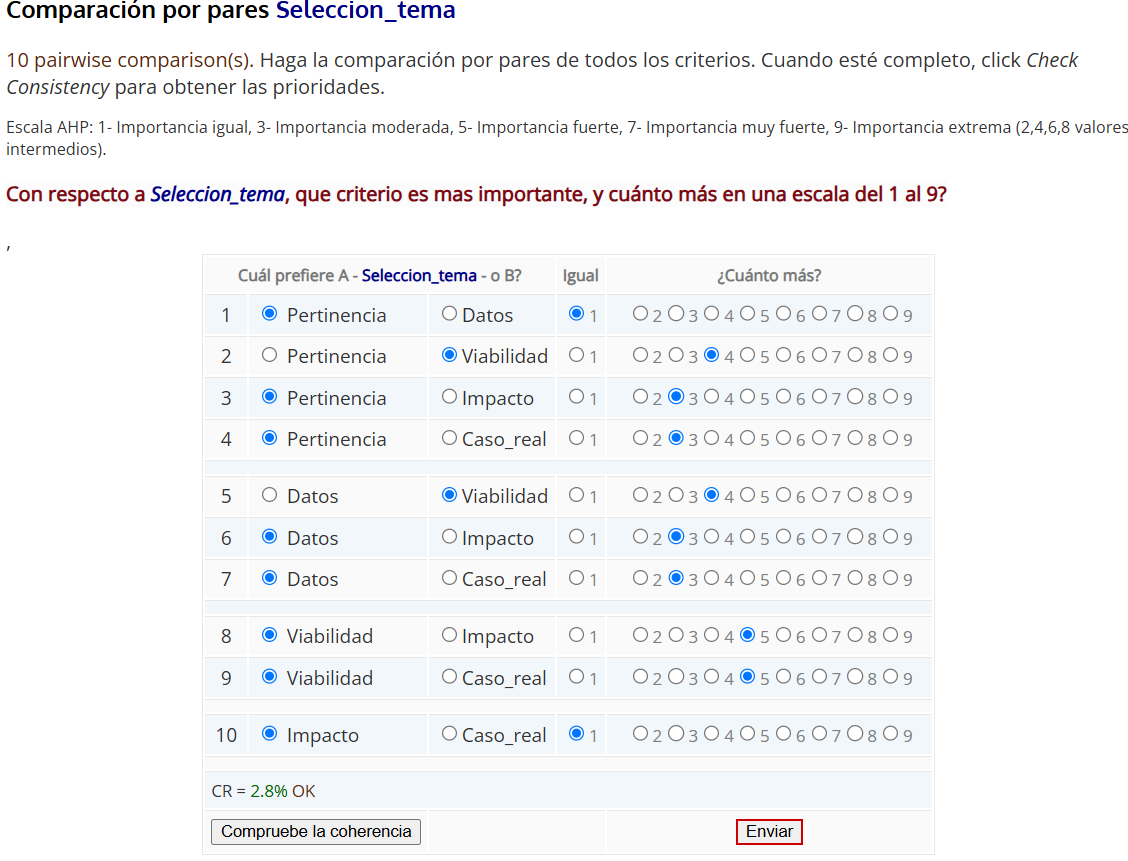
\includegraphics[width=\textwidth]{criterios_ahp.png}
\caption{Comparación por pares de los criterios y prioridades resultantes (AHP-OS).}\label{fig:criterios}
\end{figure}

\begin{table}[H]
\centering
\small
\caption{Pesos de los criterios (CR = 2,8\,\%).}\label{tab:pesos}
\begin{tabular}{@{}lcc@{}}
\toprule
Criterio & Peso (\%) & Posición\\
\midrule
Pertinencia & 17,5 & 2\\
Datos & 17,5 & 2\\
Viabilidad & 51,0 & 1\\
Impacto & 7,0 & 4\\
Caso\_real & 7,0 & 4\\
\bottomrule
\end{tabular}
\end{table}

\section{Comparación por pares de las alternativas según los criterios}

A = cadena de suministro, B = continuidad operativa y riesgos, C = planificación de producción en agroindustria.

\begin{table}[H]
\centering
\small
\caption{Criterio: pertinencia con la ingeniería industrial.}
\begin{tabular}{@{}p{2cm}p{1.1cm}p{1cm}p{7.3cm}@{}}
\toprule
Comparación & Gana & Valor & Razón\\
\midrule
A vs B & A & 2 & Inventarios, rutas y logística son más centrales en la carrera que la gestión de riesgos\\
A vs C & Igual & 1 & Ambas usan herramientas clásicas (logística, planeación)\\
B vs C & C & 2 & Pronósticos y planeación agregada son núcleo de ingeniería industrial\\
\bottomrule
\end{tabular}
\end{table}

\begin{table}[H]
\centering
\small
\caption{Criterio: disponibilidad de datos.}
\begin{tabular}{@{}p{2cm}p{1.1cm}p{1cm}p{7.3cm}@{}}
\toprule
Comparación & Gana & Valor & Razón\\
\midrule
A vs B & Igual & 1 & Las dos dependen de datos internos de una empresa\\
A vs C & C & 3 & Hay datos públicos de clima (índice ONI, servicios meteorológicos) y de producción agrícola\\
B vs C & C & 3 & Mismo motivo: B necesita historial de incidentes de una planta, difícil de conseguir\\
\bottomrule
\end{tabular}
\end{table}

\begin{table}[H]
\centering
\small
\caption{Criterio: viabilidad en tiempo y recursos.}
\begin{tabular}{@{}p{2cm}p{1.1cm}p{1cm}p{7.3cm}@{}}
\toprule
Comparación & Gana & Valor & Razón\\
\midrule
A vs B & B & 2 & B se limita a una planta; A involucra varios actores (proveedores, transporte)\\
A vs C & C & 4 & C se puede hacer con series históricas y software común\\
B vs C & C & 2 & B exige planes validados con personal de toda la planta, C se limita a la producción y demanda\\
\bottomrule
\end{tabular}
\end{table}

\begin{table}[H]
\centering
\small
\caption{Criterio: impacto económico y social.}
\begin{tabular}{@{}p{2cm}p{1.1cm}p{1cm}p{7.3cm}@{}}
\toprule
Comparación & Gana & Valor & Razón\\
\midrule
A vs B & A & 4 & Una disrupción en la cadena de suministro afecta a proveedores, transportistas, distribuidores, comercios y consumidores finales; la continuidad operativa protege principalmente a una sola planta y a sus trabajadores\\
A vs C & A & 2 & Ambos tienen alcance regional, pero la cadena de suministro conecta a más eslabones y sectores, mientras que la planificación agroindustrial se concentra en productores y procesadores del sector agrícola\\
B vs C & C & 2 & La planificación de producción agroindustrial beneficia a varios productores y a los precios de la zona, mientras que B se limita a una planta\\
\bottomrule
\end{tabular}
\end{table}

\begin{table}[H]
\centering
\small
\caption{Criterio: acceso a un caso de estudio real.}
\begin{tabular}{@{}p{2cm}p{1.1cm}p{1cm}p{7.3cm}@{}}
\toprule
Comparación & Gana & Valor & Razón\\
\midrule
A vs B & B & 2 & Es más fácil entrar a una sola planta que mapear una cadena completa\\
A vs C & C & 4 & Hay muchas empresas, cooperativas y productores agroindustriales\\
B vs C & C & 2 & Las plantas suelen ser reservadas con información de riesgos\\
\bottomrule
\end{tabular}
\end{table}

La consistencia de los juicios se verificó con la razón de consistencia (CR) de Saaty, que debe ser menor a 0,10. La matriz de comparación de criterios obtuvo un CR de 2,8\,\%, y las cinco matrices de alternativas (una por criterio) obtuvieron un CR de 0\,\%, por lo que todos los juicios son aceptables.

\section{Resultados}

La Tabla~\ref{tab:jerarquia} presenta las prioridades locales de cada alternativa y su prioridad global (peso del criterio por prioridad local).

El ranking final es:
\begin{enumerate}
\item \textbf{C: Planificación de producción en agroindustria, 52,6\,\%.}
\item B: Continuidad operativa y riesgos, 24,6\,\%.
\item A: Cadena de suministro, 22,8\,\%.
\end{enumerate}

\begin{table}[H]
\centering
\footnotesize
\caption{Prioridades locales (L) y globales (G, en \%) por criterio.}\label{tab:jerarquia}
\setlength{\tabcolsep}{4pt}
\begin{tabular}{@{}lcccccccc@{}}
\toprule
 & & \multicolumn{2}{c}{A} & \multicolumn{2}{c}{B} & \multicolumn{2}{c}{C}\\
\cmidrule(lr){3-4}\cmidrule(lr){5-6}\cmidrule(lr){7-8}
Criterio & Peso & L & G & L & G & L & G\\
\midrule
Pertinencia & 0,175 & 0,400 & 7,0 & 0,200 & 3,5 & 0,400 & 7,0\\
Datos & 0,175 & 0,200 & 3,5 & 0,200 & 3,5 & 0,600 & 10,5\\
Viabilidad & 0,510 & 0,143 & 7,3 & 0,286 & 14,6 & 0,571 & 29,1\\
Impacto & 0,070 & 0,571 & 4,0 & 0,143 & 1,0 & 0,286 & 2,0\\
Caso\_real & 0,070 & 0,143 & 1,0 & 0,286 & 2,0 & 0,571 & 4,0\\
\midrule
\textbf{Total} & 1,000 & & \textbf{22,8} & & \textbf{24,6} & & \textbf{52,6}\\
\bottomrule
\end{tabular}
\end{table}

C duplica a los otros dos, mientras que B y A quedan casi empatados. C gana sobre todo por viabilidad, donde aporta 29,1 de sus 52,6 puntos. También gana en datos (10,5\,\%) y empata con A en pertinencia (7,0\,\%). A solo lidera en impacto (4,0\,\%), un criterio de apenas 7\,\%, y por eso no alcanza. B se sostiene casi solo por viabilidad (14,6\,\%).

\begin{figure}[H]
\centering
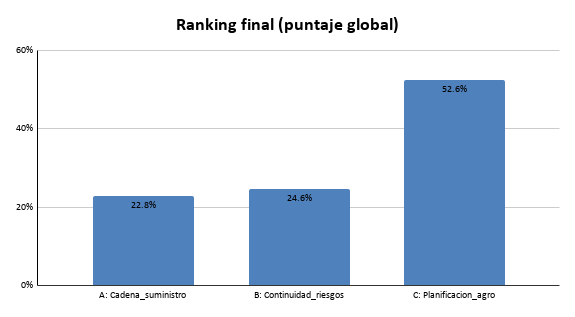
\includegraphics[width=0.85\textwidth]{ranking.png}
\caption{Ranking final (puntaje global).}\label{fig:ranking}
\end{figure}

\begin{figure}[H]
\centering
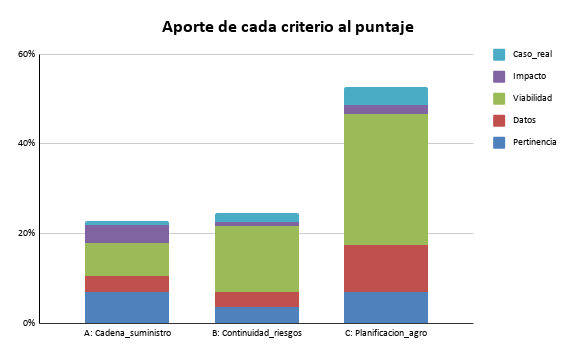
\includegraphics[width=0.85\textwidth]{aporte.png}
\caption{Aporte de cada criterio al puntaje global de cada tema.}\label{fig:aporte}
\end{figure}

\section{Análisis de sensibilidad}

Los pesos del AHP surgen de juicios subjetivos, por lo que se evaluó si el tema ganador se mantiene cuando esos pesos cambian. Además del escenario base, se probaron cinco escenarios alternativos: (1) \emph{Viabilidad baja}, como si el tiempo y los recursos fueran menos restrictivos; (2) \emph{Pesos iguales}; (3) \emph{Impacto alto}; (4) \emph{Caso real alto}; y (5) \emph{Sin Viabilidad}, donde este criterio se elimina (0\,\%) para simular que no hubiera restricciones de tiempo y recursos. Estos escenarios son supuestos propuestos para explorar el modelo y no provienen de datos externos.

\begin{table}[H]
\centering
\footnotesize
\caption{Escenarios de ponderación (pesos y puntajes en \%).}\label{tab:escenarios}
\setlength{\tabcolsep}{3pt}
\resizebox{\textwidth}{!}{%
\begin{tabular}{lccccccccccc}
\toprule
 & \multicolumn{5}{c}{Peso del criterio} & \multicolumn{3}{c}{Puntaje} & & \\
\cmidrule(lr){2-6}\cmidrule(lr){7-9}
Escenario & Per. & Datos & Viab. & Imp. & Caso & A & B & C & Ganador & Margen\\
\midrule
Base (AHP) & 17,5 & 17,5 & 51,0 & 7,0 & 7,0 & 22,8 & 24,6 & 52,6 & C & 28,1\\
Viabilidad baja & 25,0 & 25,0 & 30,0 & 10,0 & 10,0 & 26,4 & 22,9 & 50,7 & C & 24,3\\
Pesos iguales & 20,0 & 20,0 & 20,0 & 20,0 & 20,0 & 29,1 & 22,3 & 48,6 & C & 19,4\\
Impacto alto & 15,0 & 15,0 & 30,0 & 30,0 & 10,0 & 31,9 & 21,7 & 46,4 & C & 14,6\\
Caso real alto & 15,0 & 15,0 & 30,0 & 10,0 & 30,0 & 23,3 & 24,6 & 52,1 & C & 27,6\\
Sin Viabilidad & 30,0 & 30,0 & 0,0 & 20,0 & 20,0 & 32,3 & 20,6 & 47,1 & C & 14,9\\
\bottomrule
\end{tabular}}
\end{table}

\begin{figure}[H]
\centering
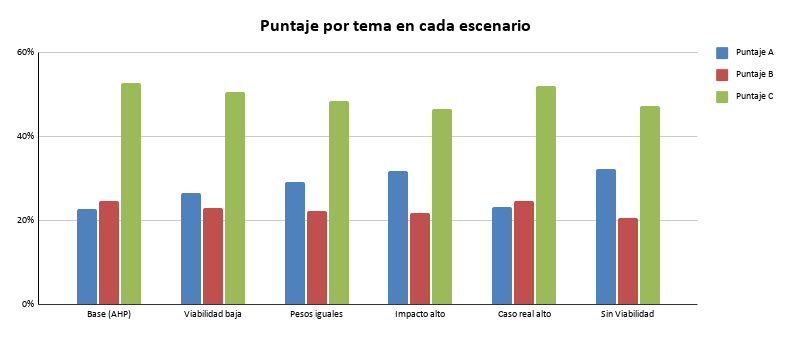
\includegraphics[width=0.95\textwidth]{escenarios.png}
\caption{Puntaje por tema en cada escenario de ponderación.}\label{fig:escenarios}
\end{figure}

\begin{table}[H]
\centering
\small
\caption{Peso crítico: peso que debería alcanzar un criterio para que otro tema supere a C.}\label{tab:critico}
\begin{tabular}{@{}lcccc@{}}
\toprule
Criterio & Peso base (\%) & Rival A & Rival B & ¿Robusto?\\
\midrule
Pertinencia & 17,5 & No cambia & No cambia & Sí\\
Datos & 17,5 & No cambia & No cambia & Sí\\
Viabilidad & 51,0 & No cambia & No cambia & Sí\\
Impacto & 7,0 & 54,5\,\% & No cambia & Cambia al llegar al peso crítico\\
Caso\_real & 7,0 & No cambia & No cambia & Sí\\
\bottomrule
\end{tabular}
\end{table}

El tema C (planificación de la producción y pronóstico de demanda en agroindustria) resultó ganador en los seis escenarios, con un puntaje entre 46,4\,\% y 52,6\,\% y un margen mínimo de 14,6 puntos sobre el segundo tema, que se dio en el escenario \emph{Impacto alto}. El análisis de peso crítico, que modifica el peso de un criterio entre 0\,\% y 100\,\% mientras los demás se reajustan proporcionalmente, indica que en cuatro de los cinco criterios ningún valor cambia el ganador. La única excepción es el impacto económico y social: el tema A (cadena de suministro) superaría a C solo si ese criterio pesara más de 54,5\,\%, frente a su peso base de 7\,\%, un valor muy poco realista para este proyecto. En consecuencia, la selección del tema C es robusta ante variaciones razonables de los juicios del decisor.

\section{Conclusión}

Aplicando el proceso analítico jerárquico (AHP) a tres temas candidatos y cinco criterios, se seleccionó como tema del proyecto final la \textbf{planificación de la producción y el pronóstico de demanda en agroindustria bajo variabilidad climática asociada al Superniño}, con un puntaje global de 52,6\,\%, frente a 24,6\,\% de la continuidad operativa y gestión de riesgos y 22,8\,\% de la resiliencia de la cadena de suministro. La ventaja de este tema se explica principalmente por su viabilidad (29,1 de sus 52,6 puntos) y por la disponibilidad de datos públicos climáticos y productivos. El análisis de sensibilidad confirmó que el resultado se mantiene bajo seis configuraciones de pesos. Como limitación, los juicios son subjetivos y reflejan el contexto del autor; se recomienda validarlos con el asesor y con expertos del sector.

\begin{thebibliography}{8}
\bibitem{saaty1980}
Saaty, T.L.: The Analytic Hierarchy Process. McGraw-Hill, New York (1980)

\bibitem{goepel2018}
Goepel, K.D.: Implementation of an online software tool for the analytic hierarchy process (AHP-OS). Int. J. Analytic Hierarchy Process \textbf{10}(3), 469--487 (2018)
\end{thebibliography}

\end{document}